\documentclass[10pt,xcolor={table,dvipsnames}]{beamer} 		% carica automaticamente amsthm, amssymb, amsmath, graphicx
\setbeamertemplate{theorems}[numbered]%[ams style] 
\setbeamertemplate{bibliography item}{\insertbiblabel}

\usepackage[T1]{fontenc}				% codifica dei font
\usepackage[utf8]{inputenc}				% lettere accentate da tastiera
\usepackage[italian]{babel}				% lingua del documento
\usepackage[italian]{varioref}			% Per usare il comando \vref{label}, che dà dei collegamenti più dettagliati

% Load the custom style file
\usepackage{AndreaStyle}
% The file `AndreaStyle.sty` is stored in: `D:\Programmi e Applicazioni\texlive\texmf-local\tex\latex\local` for Windows.
% The file `AndreaStyle.sty` is stored in: `/usr/local/texlive/texmf-local/tex/latex/local` for Ubuntu (desktop).
% This won't work in Overleaf, until the AndreaStyle.sty file is added to the project

\usepackage{mathdots}

%\usepackage{algorithm}
%\usepackage[beginLComment=//~,endLComment=~]{algpseudocodex}			% Package for typesetting algorithms

\usepackage{mathrsfs}					% Per dei caratteri matematici migliori: \mathscr{} e \mathcal{}
%\usepackage{braket} 					% Per il comando \Set, e altre (poche) cose
%\usepackage{textcomp}					% Dovrebbe aggiungere più simboli
\usepackage{bbm}						% Più simboli in \mathbb

\usepackage{fontawesome5}				% Aggiunge simboli da FontAwesome

\usepackage{hyperref}					% Importante: hyperref va caricato nel documento.


%\setcounter{tocdepth}{1}	% profondità dell'indice

	    % TEOREMI CUSTOM:
\theoremstyle{plain}					% Definisce ambienti per Teoremi, esercizi, corollari... Con lo stile adeguato
	\newtheorem{proposizione}{Proposizione}%[section]
	\newtheorem*{proposizione*}{Proposizione}
	
	\newtheorem{teorema}{Teorema}%[section]
	\newtheorem*{teorema*}{Teorema}
		
	%\newtheorem{lemma_es}{Lemma}[esercizio]
	%\newtheorem{lemma}{Lemma}[section]
	\newtheorem*{lemma*}{Lemma}
	\newtheorem{corollario}{Corollario}[section]


\theoremstyle{definition}				
	\newtheorem{definizione}{Definizione}%[section]%[chapter]
	\newtheorem*{definizione*}{Definizione}	%definizione non numerata
	\newtheorem*{notazione}{Notazione}

\theoremstyle{remark}
	\newtheorem{oss}{Osservazione}%[section]
	\newtheorem*{oss*}{Osservazione}


    	% COMANDI CUSTOM
% Define the \indicator command
\NewDocumentCommand{\indicator}{O{t} O{m} O{i}}{%
\mathlarger{\mathbbm{1}}\qty{\scriptstyle {x}_{#1}^{#2}=#3}%
}
% Define the \transpose command
\newcommand{\transpose}[1]{\prescript{t}{}{#1}}
% Define the \Var command, for the variance
\newcommand{\Var}[1]{\operatorname{Var}\qty(#1)}
% Define the \Cov command, for the covariance
\newcommand{\Cov}[1]{\operatorname{Cov}\qty(#1)}

% Define a command to create unnumbered footnotes
\let\svthefootnote\thefootnote
\textheight 1in
\newcommand\blankfootnote[1]{%
\let\thefootnote\relax\footnotetext{#1}%
\let\thefootnote\svthefootnote%
}
% Define the \independent symbol, for independence
\newcommand\independent{\protect\mathpalette{\protect\independenT}{\perp}}
  \def\independenT#1#2{\mathrel{\rlap{$#1#2$}\mkern2mu{#1#2}}}


\usetheme{Madrid}

\title[Seminario MNCM]{Slide di appoggio}			%WIP
%\subtitle{Presentazione e dimostrazione della convergenza} 
\author{Andrea Marino}
\institute[DI UniPi]{Università di Pisa}
%\titlegraphic{\includegraphics[width=2cm]{Immagini/cherubino_black.eps}}
\date[\today]{Metodi Numerici per le Catene di Markov\newline Seminario di fine corso}


% Custom command to insert the summary frame
\newcommand{\insertSummaryFrame}{
    \begin{frame}
        \frametitle{Sommario}
        \tableofcontents[currentsection, subsectionstyle=show/shaded/hide]
    \end{frame}
}

% Show summary at the beginning of each section
\AtBeginSection[]
{
    \begin{frame}
        \frametitle{Sommario}
        \tableofcontents[currentsection, subsectionstyle=show/hide/hide]
    \end{frame}
}

% Show summary at the beginning of each subsection
\AtBeginSubsection[]
{
    \begin{frame}
        \frametitle{Sommario}
        \tableofcontents[currentsection, subsectionstyle=show/shaded/hide]
    \end{frame}
}

\begin{document}
    \begin{frame}[plain]
        \titlepage
    \end{frame}

\section*{Sommario}
	\setcounter{tocdepth}{1}
	\begin{frame}
		\frametitle{Sommario}
		\tableofcontents
	\end{frame}
	
	\setcounter{tocdepth}{2}  
    
\section{Analisi teorica}

    \begin{frame}
        {\hypertarget{frame:teorema_1_part1}{$\hat{P}_{\textup{MoM}}$ è consistente$\qquad 1/3$}}

        Supponiamo che:
        \begin{enumerate}
            \item $\pi_0=\pi$, ossia $\qty{x_t^{(m)}}_{t\in[T]}$ è \emph{fortemente} stazionario
            \item<2-> $\P{\vb*{y}}{\vb*{n}}$ rispetti le ipotesi della proposizione~\ref{prop:noise_model}
            \item<3-> $N\in\mathbb{N}, A\in\R{S}{S}$ siano noti {\smaller (e costanti: forte stazionarietà $\implies A_t=A\quad\forall\,t\in[T]$)}
        \end{enumerate}

        \begin{teorema}<4->\label{teor:consistenza_P_mom}
            Sia $\hat{P}_{T,K}$ lo stimatore restituito dall'algoritmo per il caso stazionario.

            Nelle ipotesi precedenti, $\hat{P}_{T,K}$ è consistente.%, ossia converge in probabilità 
            %a $P$ per $T\to\infty$ e/o $K\to\infty$.
        \end{teorema}
        \begin{block}<5->{Dimostrazione.}
            \begin{itemize}
                \item ${K\to\infty}$
                \begin{itemize}
                    \item<5-> Per la legge dei grandi numeri, $\lim_K\hat{\vb*{m}}_t=\mathbb{E}\qty[\vb*{y}_t]$ q.c.
                    \onslide<6->{Dunque 
                    $\lim_K\hat{\vb*{m}}=\lim_k\frac{1}{T}\sum_{t=1}^T\hat{\vb*{m}}_t=\mathbb{E}\qty[\vb*{y}_1]$ q.c.
                    (cfr. Appendice~\hyperlink{frame:teorema1_lim_mhat:appencide}{\faHandPointRight})}
                    \item<7-> Similmente si dimostra che $\lim_K\hat{\Sigma}_{t,t+1}=\Cov{\vb*{y}_1,\vb*{y}_2}$ q.c.
                    e dunque $\hat{\Sigma}=\frac{1}{T-1}\sum_{t=1}^{T-1}\hat{\Sigma}_{t,t+1}\overset{K\to\infty}{\longrightarrow}\Cov{\vb*{y}_1,\vb*{y}_2}$ q.c.
                    (cfr. Appendice~\hyperlink{frame:teorema1_lim_Sigmahat:appendice}{\faHandPointRight})
                \end{itemize}
                \onslide<8->{Ma allora $\hat{P}_{T,K}\xrightarrow{K\to\infty}P$ in probabilità.}
            \end{itemize}
        \end{block}
    \end{frame}

    \begin{frame}
        {\hypertarget{frame:teorema_1_part2}{$\hat{P}_{\textup{MoM}}$ è consistente$\qquad 2/3$}}

        \begin{block}{}
            \begin{itemize}
                \item $T\to\infty$
                
                Possiamo supporre $K=1$. Dunque $\hat{\vb*{m}}_t=\vb*{y}_t$ e $\hat{\vb*{m}}=\frac{1}{T}\sum_{t=1}^{T}\vb*{y}_t$. \onslide<2->{Dobbiamo dimostrare che (in probabilità)
                \begin{gather*}
                    \hat{\vb*{m}}\xrightarrow{T\to\infty}\mathbb{E}\qty[\vb*{y}_1],\text{ e }\\
                    \hat{\Sigma}\coloneqq\frac{1}{T-1}\sum_{t=1}^{T-1}\qty(\vb*{y}_t-\hat{\vb*{m}})\cdot\transpose{\qty(\vb*{y}_{t+1}-\hat{\vb*{m}})}\xrightarrow{T\to\infty}\Cov{\vb*{y}_1,\vb*{y}_2}
                \end{gather*}}
                %in probabilità.
                \vspace{-\baselineskip}
                
                \hspace*{.05\linewidth}\begin{minipage}{.9\linewidth}
                    \begin{definizione*}<3->
                        $\qty{X_t}_{t\in[T]}$ {\smaller (fortemente stazionario)} è detto \emph{mean-ergodic} se $\frac{1}{T}\sum_{t=1}^TX_t$ converge in media seconda alla media della popolazione $\mathbb{E}\qty[X_t]$. 
                    \end{definizione*}
                    \begin{oss*}<4->
                        Convergenza in media seconda $\implies$ convergenza in probabilità.
                    \end{oss*}
                \end{minipage}
            \end{itemize}
        \end{block}

    \end{frame}

    \begin{frame}
        {\hypertarget{frame:teorema_1_part3}{$\hat{P}_{\textup{MoM}}$ è consistente$\qquad 3/3$}}

        \begin{block}{}
            ${\vb*{y}}_t$ 
            mean-ergodic vuol dire che $\frac{1}{T}\sum_{t=1}^T\vb*{y}_t\xrightarrow{T\to\infty}\mathbb{E}\qty[\vb*{y}_1]$.
            \onslide<2->{Similmente, $\hat{\Sigma}\xrightarrow{T\to\infty}\Cov{\vb*{y}_1,\vb*{y}_2}$ se il processo $\qty{\vb*{Z}_t}_{t\in[T-1]}$, $\vb*{Z}_t\coloneqq\vb*{y}_t\cdot\transpose{\vb*{y}_{t+1}}$, è mean-ergodic.}

            \onslide<3->{Per dimostrarlo, è sufficiente dimostrare che $\qty{\vb*{Z}_t(i,j)}_{t\in[T-1]}$ è 
            mean-ergodic $\quad$ ({\smaller $\vb*{Z}_t(i,j)=\vb*{y}_{t}(i)\vb*{y}_{t+1}(j)$}).}
            
            \hspace{.05\linewidth}\begin{minipage}{.9\linewidth}
                \begin{block}<4->{Proposizione {\smaller~\cite[Theorem 12.2 (p.~528)]{book:Papoulis}}}
                    Sia $\qty{X_t}_{t\in[T]}$ stazionario e sia $\gamma_X(\tau)\coloneqq\Cov{X_{t+\tau},X_t}$ la sua funzione di autocovarianza. Se $\lim_{\tau\to\infty}\gamma_X(\tau)=0$ allora $\qty{X_t}_{t\in[T]}$ è mean-ergodic. 
                \end{block}                
            \end{minipage}
            \medskip
            
            \begin{enumerate}
                \item<5-> Consideriamo i processi $\qty{\vb*{n}_t}_{t\in[T]}$ e $\qty{z_t(i,j)}_{t\in[T-1]}$, $z_t(i,j)\coloneqq\vb*{n}_t(i)\vb*{n}_{t+1}(j)$ 
                \item<6-> Si dimostra che $\gamma_{\vb*{n}}(\tau)\xrightarrow{\tau\to\infty}0$ {\smaller (cfr. Appendice~\hyperlink{frame:teorema1_lim_gamma_n:appendice}{\faHandPointRight})} e che $\gamma_z(i,j)\xrightarrow{\tau\to\infty}0$
                \item<7-> Si dimostra che $\qty{\vb*{n}_t}_{t\in[T]}$ mean-ergodic $\implies\qty{\vb*{y}_t}_{t\in[T-1]}$ mean-ergodic {\smaller (cfr. Appendice~\hyperlink{frame:teorema1_yt_tp1_mean_ergodic:appendice}{\faHandPointRight})}
                \item<8-> Si dimostra che $\qty{z_t(i,j)}_{t\in[T-1]}$ mean-ergodic $\implies\qty{\vb*{Z}_t(i,j)}_{t\in[T-1]}$ mean-ergodic {\smaller (cfr. Appendice~\hyperlink{frame:teorema1_yt_mean_ergodic:appendice}{\faHandPointRight})}.\onslide<8->{\hfill$\square$}
            \end{enumerate}
        \end{block}
        
    \end{frame}


  
\section{Esperimenti numerici}
    \begin{frame}{Rischio degli stimatori}
        \begin{teorema}
            Per $TK\to\infty$, gli stimatori $\hat{\vb*{m}}$ e $\hat{\Sigma}$ sono non distorti, e hanno varianza (dunque rischio quadratico) $O(1/TK)$. 
        \end{teorema}
        \begin{proof}<2->
            La dimostrazione si ottiene adattando quella del teorema~\ref{teor:consistenza_P_mom} e usando~\cite[12-12 (p.~528)]{book:Papoulis}. Maggiori dettagli in~\cite{article:main}.
        \end{proof}
        \medskip

        \onslide<3->{Un'analisi teorica del rischio di $\hat{P}_{\textup{MoM}}$ non è stata svolta in~\cite{article:main}.} 
        
        \onslide<4->{Gli autori hanno presentato risultati empirici che suggeriscono che anche l'errore quadratico medio di $\hat{P}_{\textup{MoM}}$ sia $O(1/TK)$.}
    \end{frame}

    \begin{frame}
        {Esperimenti numerici}
        {MSE vs. \texorpdfstring{$T\times K$}{TxK}, algoritmo per il calcolo di $\hat{P}_{\textup{MoM}}$ {\smaller (caso stazionario)}}
        \begin{figure}[ht]
			\centering
			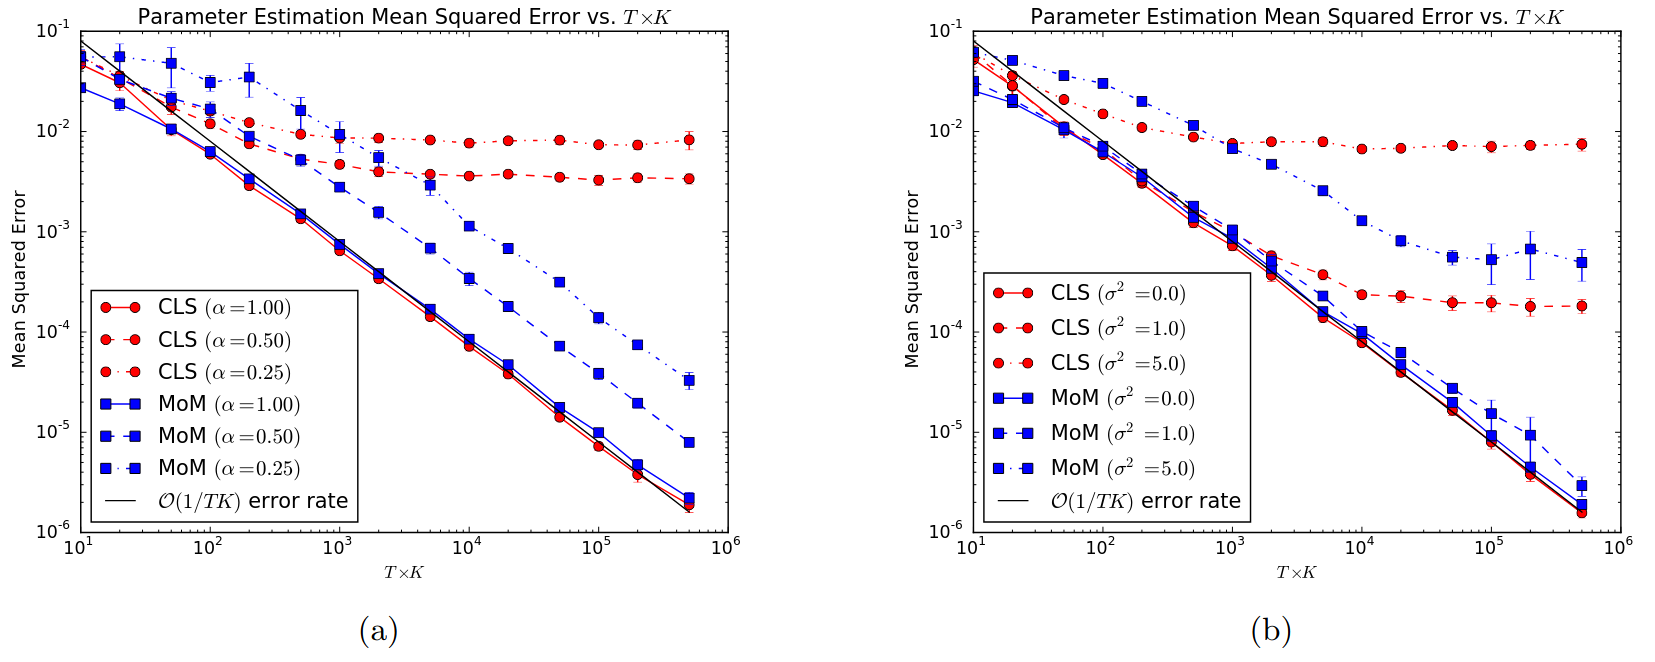
\includegraphics[width=\textwidth]{Immagini/mom_cls_results_authors.png}
			%\caption{\emph{MSE per la stima di $\hat{P}_{\textup{MoM}}$}, con errore}
		\end{figure}
        \begin{description}
            \item[(a)] $\vb*{y}_t(i)\mid\vb*{n}_t(i)\sim\mathrm{Binomial}\qty(\vb*{n}_t(i),\alpha)\quad\alpha\in[0,1]$
            \item[(b)] $\vb*{y}_t=\vb*{n}_t+\epsilon_t\quad\epsilon_t\sim\mathcal{N}\qty(0,\sigma^2)$
        \end{description}

        L'errore è dato da $\frac{1}{S^2}\norm*{\hat{P}-P}_F^2$.         
        {\smaller (Per una discussione più approfondita, cfr.~\cite{article:main})}.
    \end{frame}

    

	\begin{frame}{\refname}
		\begin{thebibliography}{9}
			\bibitem{article:main} Garrett Bernstein, Daniel Sheldon
			\newblock Consistently Estimating Markov Chains with Noisy Aggregate Data
			\newblock Proceedings of the 19th International Conference on Artificial Intelligence and Statistics, \emph{PMLR}, vol. 51, pp. 1142-1150, PMLR (2016) 09-11 May

			\bibitem{book:Norris} J. R. Norris
			\newblock Markov Chains
			\newblock Cambridge University Press, 1997

			\bibitem{book:Berger_Casella} R. L. Berger, G. Casella
			\newblock Statistical Inference (2nd ed.)
			\newblock Chapman and Hall/CRC, 2024

			\bibitem{book:Papoulis} A. Papoulis, S. U. Pillai
			\newblock Probability, Random Variables and Stochastic Processes (4th ed.)
			\newblock McGraw-Hill, 2002
		\end{thebibliography}
	\end{frame}





% ---------------------------------------------------------------------------------------
% -------------------------------------- APPENDICE --------------------------------------
% ---------------------------------------------------------------------------------------

\section*{Appendice}
	\begin{frame}
		\begin{center}
			\Huge{\textbf{Appendice}}
		\end{center}
	\end{frame}


    \begin{frame}
        {Consistenza di \texorpdfstring{$\hat{P}_{T,K}$}{P_T,K} per \texorpdfstring{$K\to\infty$}{K tendente a infinito}$\qquad 1/2$}
        {\hypertarget{frame:teorema1_lim_mhat:appencide}{Dettagli sul calcolo di \texorpdfstring{$\lim_K\hat{\vb*{m}}$}{un limite}}}

        %\begin{block}{}
        Nel calcolo di $\lim_K\hat{\vb*{m}}$ si fa uso dell'ipotesi di stazionarietà:
        \begin{align*}
            \lim_K\hat{\vb*{m}}&=\lim_K\frac{1}{T}\sum_{t=1}^T\hat{\vb*{m}}_t=\frac{1}{T}\sum_{t=1}\
            \lim_K\hat{\vb*{m}}_t=\frac{1}{T}\sum_{t=1}^T\mathbb{E}\qty[\vb*{y}_t]\
            =\frac{1}{T}\sum_{t=1}^T A_t\mathbb{E}\qty[\vb*{n}_t]\\
        \intertext{Per ipotesi $A_t=A\quad\forall\,t\in[T]$. Dunque}
            &=\frac{1}{T}\cdot A\cdot\sum_{t=1}^T\mathbb{E}\qty[\vb*{n}_t]=\frac{1}{T}\cdot A\cdot T\cdot\mathbb{E}\qty[\vb*{n}_1]=A\cdot\mathbb{E}\qty[\vb*{n}_1]=\mathbb{E}\qty[\vb*{y}_1]
        %\intertext{Ma per stazionarietà $\mathbb{E}\qty[\vb*{n}_t]=\mathbb{E}\qty[\vb*{n}_1]\quad\forall\,t\in[T]$. Dunque}
        \end{align*}
        poiché per stazionarietà $\mathbb{E}\qty[\vb*{n}_t]=\mathbb{E}\qty[\vb*{n}_1]\quad\forall\,t\in[T]$.
        %\end{block}

        \blankfootnote{\textbf{Indietro:}~\hyperlink{frame:teorema_1_part1}{\faHandPointLeft}}
    \end{frame}

    \begin{frame}
        {Consistenza di \texorpdfstring{$\hat{P}_{T,K}$}{P_T,K} per \texorpdfstring{$K\to\infty$}{K tendente a infinito}$\qquad 2/2$}
        {\hypertarget{frame:teorema1_lim_Sigmahat:appendice}{Dettagli sul calcolo di \texorpdfstring{$\lim_k\hat{\Sigma}_{t,t+1}$}{un altro limite}}}

        %\begin{block}{}
        Consideriamo 
        \[
            \hat{\Sigma}_{t,t+1}=\frac{1}{K}\sum_{k=1}^{K}\qty(\vb*{y}_t^{(k)}-\hat{\vb*{m}}_t)\cdot\transpose{\qty(\vb*{y}_{t+1}^{(k)}-\hat{\vb*{m}}_{t+1})}=\frac{1}{K}\sum_{k=1}^{K}\qty(\vb*{y}_t^{(k)}\cdot\transpose{\vb*{y}}_{t+1}^{(k)})-\hat{\vb*{m}}_t\cdot\transpose{\hat{\vb*{m}}_{t+1}}
        \]
        Per la legge dei grandi numeri $\hat{\vb*{m}}_t\xrightarrow{K\to\infty}\mathbb{E}\qty[\vb*{y}_t]$ q.c.,
        e $\frac{1}{K}\sum_{k=1}^K\vb*{y}_t^{(k)}\cdot\transpose{\vb*{y}}_{t+1}^{(k)}\xrightarrow{K\to\infty}\mathbb{E}\qty[\vb*{y}_t\cdot\transpose{\vb*{y}_{t+1}}]$ q.c.
        \medskip

        Dunque {\smaller (due applicazioni del teorema di Slusky~\cite[Theorem~5.5.17]{book:Berger_Casella})} $\hat{\vb*{m}}_t\cdot\transpose{\hat{\vb*{m}}}_{t+1}\xrightarrow{K\to\infty}\mathbb{E}\qty[\vb*{y}_t]\cdot\mathbb{E}\qty[\transpose{\vb*{y}}_{t+1}]$ in legge. Ma il valore atteso è una costante, quindi la convergenza è in probabilità. 

        Poiché la convergenza quasi certa implica quella in probabilità, si ha che 
        \[
            \hat{\Sigma}_{t,t+1}\xrightarrow{K\to\infty}\mathbb{E}\qty[\vb*{y}_t\cdot\transpose{\vb*{y}_{t+1}}]-\mathbb{E}\qty[\vb*{y}_t]\cdot\mathbb{E}\qty[\transpose{\vb*{y}}_{t+1}]=\Cov{\vb*{y}_1,\vb*{y}_2}
        \]
        in quanto per stazionarietà $\Cov{\vb*{y}_t,\vb*{y}_{t+1}}=\Cov{\vb*{y}_1,\vb*{y}_2}\quad\forall\,t\in[T]$.
        %\end{block}

        \blankfootnote{\textbf{Indietro:}~\hyperlink{frame:teorema_1_part1}{\faHandPointLeft}}
    \end{frame}

    \begin{frame}
        {Consistenza di \texorpdfstring{$\hat{P}_{T,K}$}{P_T,K} per \texorpdfstring{$T\to\infty$}{T tendente a infinito}$\qquad 1/3$}
        {\hypertarget{frame:teorema1_lim_gamma_n:appendice}{Dimostrazione di $\lim_{\tau}\gamma_{\vb*{n}}(\tau)=0$}}

        %\begin{block}{}
        Consideriamo $\qty(\gamma_{\vb*{n}}(\tau))_i=\Cov{\vb*{n}_t(i),\vb*{n}_{t+\tau}(i)}\equiv\gamma_{\vb*{n}(i)}(\tau)$.
        \begin{align*}
            \gamma_{\vb*{n}(i)}(\tau)&=\operatorname{Cov}\bigg(\sum_{m=1}^N\indicator,\sum_{m'=1}^N\indicator[t+\tau][m'][i]\bigg)\\
            %\begin{aligned}[t]
            &=\sum_{m=m'}\Cov{\indicator,\indicator[t+\tau][m][i]}+\sum_{m\ne m'}\cancel{\Cov{\indicator,\indicator[t+\tau][m'][i]}}\\
            %\end{aligned}\\
            &=N\Big(\mathbb{E}\qty[\indicator\indicator[t+\tau]]-\mathbb{E}\qty[\indicator]\mathbb{E}\qty[\indicator[t+\tau]]\Big)\\
            &=N\Big(\P{x_{t+\tau}^{m}=i,x_t^{m}=i}-\P{x_t^m=i}\P{x_{t+\tau}^m=i}\Big)\\
            &=N\Big(\P{x_{t+\tau}^m=i}{x_t^{m}=i}\P{x_t^m=i}-\vb*{\mu}_t(i)\cdot\vb*{\mu}_{t+\tau}(i)\Big)\\
            &=N\vb*{\mu}_t(i)\cdot\Big(P^{\tau}_{i,i}-\vb*{\mu}_{t+\tau}(i)\Big)\xrightarrow{\tau\to\infty}0
        \end{align*}
        in quanto per l'ergodicità $\lim_{\tau}\vb*{\mu}_{t+\tau}=\pi$ e $\lim_{\tau}P_{i,j}^{\tau}=\pi_j\quad\forall\,i,j\in[S]$.%\hfill$\square$
        %\end{block}


        \blankfootnote{\textbf{Indietro:}~\hyperlink{frame:teorema_1_part3}{\faHandPointLeft}}
    \end{frame}

    \begin{frame}
        {Consistenza di \texorpdfstring{$\hat{P}_{T,K}$}{P_T,K} per \texorpdfstring{$T\to\infty$}{T tendente a infinito}$\qquad 2/3$}
        {\hypertarget{frame:teorema1_yt_mean_ergodic:appendice}{Se \texorpdfstring{$\qty{\vb*{n}_t}_{t\in[T]}$}{n_t} è mean-ergodic, allora \texorpdfstring{$\qty{\vb*{y}_t}_{t\in[T]}$}{y_t} lo è}}

        \begin{itemize}
            \item Per la proposizione~\ref{prop:noise_model} si ha 
            \[
                \gamma_{\vb*{y}}(\tau)=\Cov{\vb*{y}_t,\vb*{y}_{t+\tau}}=A_t\cdot\qty(\Cov{\vb*{n}_t,\vb*{n}_{t+\tau}})\cdot\transpose{A}_{t+\tau}=A_t\cdot\gamma_{\vb*{n}}(\tau)\cdot\transpose{A}_{t+\tau}
            \]
            dunque $\lim_{\tau\to\infty}\gamma_{\vb*{n}}(\tau)=0\implies\lim_{\tau\to\infty}\gamma_{\vb*{y}}(\tau)=0$.
            \item Tramite la proposizione~\ref{prop:noise_model} si dimostra che 
            \[
                \Cov{\vb*{y}_s\cdot\transpose{\vb*{y}}_t,\vb*{y}_u\cdot\transpose{\vb*{y}}_v}=A_s\cdot\Cov{\vb*{n}_s\cdot\transpose{\qty(A_t\vb*{n}_t)},\qty(A_u\vb*{n}_u)\cdot\transpose{\vb*{n}}_v}\cdot\transpose{A}_v
            \]
            Inoltre per $\Cov{\vb*{n}_s\cdot\transpose{\qty(A_t\vb*{n}_t)},\qty(A_u\vb*{n}_u)\cdot\transpose{\vb*{n}}_v}_{i,j}$ si ha
            \begin{gather*}
                \operatorname{Cov}\Big(\vb*{n}_s(i)\cdot (A_t\vb*{n}_t)(j),\,(A_u\vb*{n}_u)(i)\cdot\vb*{n}_v(j)\Big)=\\
                \operatorname{Cov}\Big(\vb*{n}_s(i)\cdot\sum_{k}A_t(j,k)\vb*{n}_t(k),\,\vb*{n}_v(j)\cdot\sum_{k'}A_u(i,k')\vb*{n}_u(k')\Big)=\\
                \sum_{k,k'}A_t(j,k)\cdot A_u(i,k')\cdot\operatorname{Cov}\Big(\vb*{n}_s(i)\vb*{n}_t(k),\,\vb*{n}_u(k')\vb*{n}_v(j)\Big)
            \end{gather*}
            %\textbf{\textcolor{red}{Finire}}
        \end{itemize}

        \blankfootnote{\textbf{Indietro:}~\hyperlink{frame:teorema_1_part3}{\faHandPointLeft}}
    \end{frame}

    \begin{frame}
        {Consistenza di \texorpdfstring{$\hat{P}_{T,K}$}{P_T,K} per \texorpdfstring{$T\to\infty$}{T tendente a infinito}$\qquad 3/3$}
        {\hypertarget{frame:teorema1_yt_tp1_mean_ergodic:appendice}{Se \texorpdfstring{$\qty{\vb*{n}_t\cdot\transpose{\vb*{n}}_{t+1}}_{t\in[T]}$}{n_t n_{t+1}} è mean-ergodic, allora \texorpdfstring{$\qty{\vb*{y}_t\cdot\transpose{\vb*{y}}_{t+1}}_{t\in[T]}$}{y_t y_{t+1}} lo è}}
        
        Il caso che ci interessa è con gli istanti temporali $t\leftarrow t+1$, $s\leftarrow t$, $u\leftarrow t+\tau$, $v\leftarrow t+1+\tau$.
        \smallskip

        Modificando gli indici nella dimostrazione fornita nel materiale supplementare di~\cite{article:main}, si dimostra che 
        \[
            \lim_{\tau\to\infty}\operatorname{Cov}\Big(\vb*{n}_{t}(i)\vb*{n}_{t+1}(k),\vb*{n}_{t+\tau}(k')\vb*{n}_{t+1+\tau}(j)\Big)=0\qquad\forall\,k,k'\in[S].
        \]

        Dunque $\Cov{\vb*{n}_s\cdot\transpose{\qty(A_t\vb*{n}_t)},\qty(A_u\vb*{n}_u)\cdot\transpose{\vb*{n}}_v}_{i,j}\xrightarrow{\tau\to\infty}0\quad\forall\,i,j\in[S]$, 
        da cui segue che $\lim_{\tau\to\infty}\gamma_{\vb*{Z}}(\tau)=0$, ovvero $\qty{\vb*{y}_t\cdot\transpose{\vb*{y}}_{t+1}}_{t\in[T-1]}$ è mean-ergodic.


        \blankfootnote{\textbf{Indietro:}~\hyperlink{frame:teorema_1_part3}{\faHandPointLeft}}
    \end{frame}




\end{document}